\documentclass[10pt, conference]{IEEEtran}

\usepackage{graphicx}
\usepackage{caption}
\usepackage{subcaption}
\usepackage{indentfirst}
\usepackage{subfig}
\usepackage{amssymb}
\usepackage[cmex10]{amsmath}

\usepackage{algorithm}
\usepackage[noend]{algpseudocode}
\usepackage{setspace}
\usepackage{url}
\usepackage{cite}
\usepackage[utf8x]{inputenc}
\usepackage{multirow}

\graphicspath{{./img/}}

\setlength{\textfloatsep}{7pt}

\begin{document}

\title{Evaluation of Optimization Strategies for fastsg\\ on Heterogeneous
Systems}
% \author{\IEEEauthorblockN{Andrei Deftu}
% \IEEEauthorblockA{Technische Universit\"{a}t M\"{u}nchen\\
% andrei.deftu@in.tum.de}
% \and
% \IEEEauthorblockN{Alin Murara\c{s}u}
% \IEEEauthorblockA{Technische Universit\"{a}t M\"{u}nchen\\
% murarasu@in.tum.de}
% }

\maketitle

\noindent\makebox[\textwidth][c]{%
\begin{minipage}[t]{0.6\textwidth}
\vspace{20pt}
\noindent\hrulefill\par
\begin{abstract}
Given the existing heterogeneous processor landscape dominated by CPUs and GPUs,
topics such as programming productivity and performance portability have become
increasingly important. In this context, an important question refers to how can
we develop optimization strategies that cover both CPUs and GPUs. We answer this
for \textit{fastsg}, a library that provides functionality for handling
efficiently high-dimensional functions. As it can be employed for compressing
and decompressing large-scale simulation data, it finds itself at the core of a
computational steering application which serves us as test case. We describe our
experience with implementing \textit{fastsg}'s time critical routines for Intel
CPUs and Nvidia Fermi GPUs. We show the differences and especially the
similarities between our optimization strategies for the two architectures. With
regard to our test case for which achieving high speedups is a ``must'' for
real-time visualization, we report a speedup of up to 6.2x times compared to the
state-of-the-art implementation of the sparse grid technique for GPUs.
\end{abstract}

\begin{IEEEkeywords}
sparse grids, GPU, library, optimizations, CUDA
\end{IEEEkeywords}
\noindent\hrulefill\par
\end{minipage}
}

\clearpage

\section{Introduction}
The number of processor architectures has grown significantly in the recent
years. We saw the appearance of accelerators such a GPUs as a response to the
many obstacles met by processor architects, e.g. the frequency and memory walls.
GPUs are application specific architectures, well suited for data parallelism,
for code with regular memory access patterns such as those available in
numerical or graphics applications. Compared to CPUs, GPUs contain simpler cores
but compensate with their higher number (tens of cores compared to 4 - 8 for
CPUs). The cores operate at a lower frequency (often 1 GHz against 2 - 3 GHz for
CPUs) and are in-order, hiding the latency of the instruction pipeline by
interleaving on each core the execution of thousands of threads.

A simple abstraction for GPUs is to consider them many-core architectures, with
a large number of cores and with each core including large vector units
allowing to compute up to 32 single precision flops per cycle (64 flops for
FMAD). Compute Unified Device Architecture (CUDA) is an option for programming
Nvidia GPUs. The vector units are not directly visible in CUDA. The SIMD nature
of GPUs reveals itself when applying various optimizations, e.g. for bank
conflicts and memory access coalescing \cite{cuda}. This view of GPUs as vector
processors is at the foundation of \cite{Volkov:2008:BGT:1413370.1413402}.

When reasoning about code transformations that improve performance on a wide
range of architectures, we do not want to lose ourselves in the details of the
programming models. A high-level simplified view allows us to have more
flexibility when adapting the code to new architectures. Considering this
trade-off, our goal is therefore to develop high-level code transformations that
address common features among different devices. 
% We do not expect that the sequence of transformations remains the same. 
To simplify the porting of 
applications from one architecture to another, it is essential to determine the
common and different aspects of the architectures and map the optimizations
accordingly. As an example, CPUs and GPUs have vector units and
array-of-structures to structure-of-arrays is a transformation that often is
required by both. Given the convergence of CPUs and GPUs seen in CPUs that have
doubled the width of the SIMD units and GPUs that received 2 level coherent
caches \cite{fermi}, we expect that more transformations, e.g. for locality, to
be shared between codes for CPUs and GPUs.

To test these concepts, we consider a computational steering application, the
main goal of which is to allow for a smooth, real-time interaction with
compressed simulation data. We have two phases (or algorithms) being at the core
of the compression and decompression of the simulation data. These algorithms
are in fact based on a numerical method called the sparse grid technique which
allows for a hierarchical and efficient representation of high-dimensional
functions, similar to wavelet series. Using it, it was shown that sheer amounts
of simulation data can be managed efficiently \cite{Butnaru201156}.

For enhanced performance, it was important to benefit from the latest
developments in hardware. But starting from scratch with every hardware release
is far from being a productive approach. Instead, what we followed was to
develop optimizations for loops and data layout at the same level at which we
develop algorithms. We realized that many of the transformations we are applying
are valid for both CPUs and GPUs, considering the above mentioned view of GPUs
as vector processors. Moreover, we consider that our study is important giving
that more and more programming models are emerging and the open question is if
we can design optimizations which are portable across processor architectures.

The main contributions of our paper are as follows:

\begin{itemize}
  \item We port dimensionally truncated sparse grids algorithms on GPUs and
  report a speedup of 28.3x compared to the CPU versions.
  \item We present a study on the performance of a subset of common loop
  transformations for two different architectures, CPUs and GPUs. We describe
  the challenges met along the way and their solutions.
  \item We report speedup results that, for the considered computational
  steering application, accelerate the state-of-the-art implementation up to a
  factor of 6.2x for compression and 1.5x for decompression on GPU. 
\end{itemize}

The rest of the paper is structured as follows. In
Section~\ref{sec:related_work} we place our work in the field of application
optimizations and sparse grids and relate to previous published papers.
Section~\ref{sec:cpus_vs_gpus} highlights the similarity between CPUs and GPUs,
seen as modern processors which borrow architectural features from each other,
allowing for common optimizations to be used.
In Section~\ref{sec:optimizations} we describe a set of loop transformation
suitable for both architectures in this context. Section~\ref{sec:comp_steering}
introduces in the field of sparse grids and presents the core functionality of
our library. Section~\ref{sec:op_strategies} shows how we can apply
optimizations for both CPUs and GPUs based on the aforementioned ideas. In
Section~\ref{sec:evaluation} we present our results and show that despite using
different architectures, similarities in hardware characteristics can make
optimizing code easier. Finally, Section~\ref{sec:conclusion} concludes our
work.


\section{Related Work}
\label{sec:related_work}
A compact data structure and efficient in-place algorithms for regular sparse
grids were presented in \cite{Murarasu:2011:CDS:1941553.1941559} and further
extended to support dimensionally truncated sparse grids on CPUs in
\cite{murarasu12fastsg:}. In this paper we start from these basic algorithms for
dimensionally truncated sparse grids and implement new ones for GPUs. In
addition, we present a set of loop transformations for increasing the
performance on both CPUs and GPUs.

A set of techniques for efficient programming of hybrid systems in the context
of dense linear algebra were presented in \cite{Tomov:2010:TDL:1805333.1805388}.
Here they show how the computation can be split for a better exploitation of
each device, but do not address the problem of programming CPUs and GPUs using a
set of common features. However, we believe that auto-tuning and in particular
runtime auto-tuning would have a good support in hybrid systems in the years to
come.

Also related to this field of study is the work from
\cite{Augonnet:2011:SUP:1951453.1951454}, which shows techniques for efficiently
exploiting heterogeneous systems through an uniform execution model. This would
allow the design of kernels for executing tasks in parallel and provide some
auto-tuning through scheduling algorithms.


\section{CPUs versus GPUs}
Heterogeneous systems containing CPUs and accelerators allow us to reach higher
computational speeds while keeping power consumption at acceptable levels. The
most common accelerators nowadays, GPUs, are very different compared to
state-of-the-art general-purpose CPUs. While CPUs incorporate large caches and
complex logic for out-of-order execution, branch prediction, and speculation,
GPUs contain significantly more floating point units. They have in-order cores
which hide pipeline stalls through interleaved multithreading, e.g. allowing up
to 1536 concurrent threads per core\footnote{In Nvidia terminology a core is
called Streaming Multi-Processor.}.
Garland et al.~\cite{garland2010} refer to CPUs as latency oriented processors
with complex techniques used for extracting Instruction Level Parallelism (ILP)
from sequential programs. In contrast, GPUs are throughput oriented, containing
a large number of cores (e.g. 16) with wide SIMD units (e.g. 32 lanes), making
them ideal architectures for vectorizable codes. All applications can be run on
CPUs but only a subset can be ported to or deliver good performance on GPUs,
making them special purpose processors. In the following, we refer to GPUs and
CPUs as processors, but of different type.

Given their specific architectural characteristics, programming the CPU and the
GPU is inherently different. Multi-core CPUs are programmed using operating
system threads. For GPU programming, CUDA is also based on threads, but there
are differences. For synchronization, CUDA only provides barriers within thread
groups running on the same GPU core, and atomic operations. For performance, the
architectural details of GPUs have to be considered. Maximizing the number of
threads running concurrently on the GPU, coalescing accesses to global memory,
eliminating bank conflicts, minimizing the number of branches, and utilizing the
various memories appropriately (global, shared, texture, constant) are important
GPU optimizations. In contrast, common CPU optimizations include cache blocking
and vectorization.
% In contrast, CPU optimizations include blocking at different memory levels and
% arranging and aligning data for SSE / AVX operations.

We will describe in the following subsections the current GPU architectures
using CUDA terms and provide some brief guidelines for programming Nvidia cards.

\subsection{GPU Architecture}

In contrast to CPUs which use the die space for complex control logic and large
caches, GPUs devote a higher percentage of transistors to floating point units.
GPUs provide massive parallelism and deliver better performance than CPUs
especially for applications with regular access patterns, e.g. dense matrix
operations \cite{volkov2008}.

In the following we focus on the GeForce GTX 480 model of Nvidia Fermi.
This is a high-end GPU which contains 15 32-way SIMD units called by Nvidia
Streaming Multiprocessors (SM). In Nvidia terminology, each way is called a
Scalar Processor (SP). Each thread is generally executed on one of the 32 ways
of the SIMD unit. One of the main characteristics of Nvidia GPUs is multithreading
which offers the possibility to hide the latency originating from various
instructions, especially the latency caused by loads from and stores to RAM, by
executing a large number of threads concurrently with a low cost per context
switch.

Nvidia GPUs are SIMD based architectures. Each SM control unit creates, manages
and executes synchronously the threads in groups of 32 called warps. Every
instruction is broadcasted synchronously to all the active threads in a warp.
Branching may cause threads in the same warp to follow different execution
paths. This type of behavior of the threads inside a warp is called diverge. It
has the potential to severely reduce the performance of a GPU application, up to
a factor of 32.

GPUs have their own dedicated RAM, global memory, which is in the order of
several Gigabytes, e.g. GeForce GTX 480 has 1.5 GB of DDR3 memory. For
performance, GPUs are also equipped with multiple fast memories on the chip:
constant cache, texture cache and shared memory \cite{ryo2008}. The properties
of these fast memories vary in terms of latency, bandwidth and usage. The
constant cache is a read-only cache and, according to \cite{won2010}, its
level-1 has the lowest latency among the memories on the GPU. The texture cache
is a read-only memory used for optimizing the bandwidth rather than latency,
i.e. its latency is comparable with the one of the global memory. Finally, the
shared memory is a low latency, read-write memory, is private per SM and
controlled explicitly by the programmer.


\subsection{GPU Programming}

CUDA is one of the available frameworks for programming Nvidia GPUs. From a
programming point of view, a CUDA application has a CPU and a GPU part. The main
responsibilities of the CPU part are: allocating memory  on the GPU,
transferring data to and from the GPU over PCI Express and launching the GPU
program called kernel. A kernel cannot contain recursive functions. Each
instance of a kernel is executed by a thread. Besides being packed in warps, the
threads are also grouped in blocks of threads. This grouping is important as
only the threads inside a block can synchronize via barriers
(\emph{\_\_syncthreads}) and share data from the shared memory. Each thread has
a 2d block identifier (\emph{blockIdx}) and a 3d thread identifier
(\emph{threadIdx}). Combining the block and the thread identifiers offers the
means to uniquely identify a thread on the GPU and to assign its part from the
workload to be computed on the GPU.

A first optimization for GPU programs consists of the proper exploitation of
multithreading. This is equivalent to maximizing the number of active threads
and can be achieved by reducing the register file and shared memory consumption
per thread. Second, efficient use of the memory hierarchy can provide a
substantial speedup to GPU applications. This optimization includes at least:
enabling coalesced accesses to global memory in order to reduce the number of
memory transactions, using the fast memories on-chip and reducing the number of
bank conflicts caused by accessing the shared memory. Third, divergent branches
can serialize the execution of the threads composing a warp. To improve the
performance, the number of divergent branches needs to be minimized. Note that
these are the optimizations which proved to be relevant to our application and
they represent only a subset of the optimizations applicable to CUDA
applications. For a detailed list of optimizations we refer the reader to
\cite{cuda}.

% The number of active threads is not the same for all applications. An
% optimization direction for GPU programs consists in maximizing the number of
% active threads. This is typically achievable by reducing the register and
% shared memory consumption per thread.

% Nvidia GPUs have a Single Instruction Multiple Thread (SIMT) architecture. The
% SM's control unit creates, manages and executes synchronously the threads in
% groups of 32 called warps. Every instruction is broadcast synchronously to all
% the active threads in a warp. In this context, divergence caused by branches
% may serialize the execution of the threads composing a warp. To improve the
% performance, the number of divergent branches needs to be minimized.

% GPUs have multiple fast memories on the chip: constant cache, texture cache
% and shared memory\cite{ryo2008}. Exploiting the memory hierarchy properly is
% another direction for optimizing CUDA programs.

% GPUs have their own dedicated memory which is in the order of several
% Gigabytes, e.g. Tesla has 4 GB of memory. Minimizing the memory consumption is
% also an optimization that should be considered by a CUDA developer.

% Recursive function are not allowed on GPUs\cite{cuda}. 

\section{Computational Steering Using Sparse Grids}
\label{sec:comp_steering}

Our application is the visualization of compressed, high-dimensional data
resulting from simulations \cite{Butnaru201156}. It is a well known fact that
managing the data coming from functions with high number of dimensions has an
exponential complexity on the number of dimensions. Therefore, we compress the
data using the sparse grid technique in order to reduce its size and we
decompress it afterwards for real-time visualization. For this purpose we use
the \textit{fastsg} library presented in \cite{murarasu12fastsg:}.

The main idea behind sparse grids is that we can approximate a $D$-dimensional
function $f : \Omega \rightarrow \mathbb{R}$, where $\Omega = [0, 1]^{D}$, by
discretizing $\Omega$ and representing $f$ as a weighted sum of basis functions.
If we consider \textit{levels} $\bar{l} = (l_{1},\ldots,l_{D})$ and
\textit{index} $\bar{i} = (i_{1},\ldots,i_{D})$ vectors in $\mathbb{N}^{D}$,
then each basis function will be centered at points $\bar{x}_{\bar{l},\bar{i}} =
(x_{l_{1},i_{1}},\ldots,x_{l_{D},i_{D}}) \in \mathbb{Q}^{D}$, for which $x_{l,i}
= i \cdot 2^{-l}$, $i \in \{1,\ldots,2^{l} - 1\}$, and $i$ odd. This means that
each grid point $\bar{x}_{\bar{l},\bar{i}}$ can be uniquely identified by the
pair $(\bar{l},\bar{i})$. Thus,

\[ f \approx \sum_{\bar{x}_{\bar{l},\bar{i}}} \alpha_{\bar{l},\bar{i}} \cdot
\phi_{\bar{l},\bar{i}} \]
where $\alpha_{\bar{l},\bar{i}}$ is the weight, or hierarchical coefficient, and
$\phi_{\bar{l},\bar{i}}$ is the basis function centered at grid point
$\bar{x}_{\bar{l},\bar{i}}$. In our case, $\phi_{\bar{l},\bar{i}}$ is obtained
by multiplying $D$ one-dimensional functions $\phi_{l,i} = h(2^{l}x - i)$, where
$h$ is the standard hat function $h(x) = max(1 - |x|, 0)$:

\[ \phi_{\bar{l},\bar{i}}(\bar{x}) = \prod_{t=1}^{D} \phi_{l,i}(x_{t}) .\]

Compressing a general function represented on a full grid is done by selecting
only the function values at grid points also contained in a sparse grid. This is
reduced to computing the hierarchical coefficients, process called
\textit{hierarchization}. Decompression (or \textit{interpolation}) refers to
evaluating the function anywhere inside the domain by summing up the
contributions of the basis functions averaged by their hierarchical
coefficients. This technique also enables us to interpolate at points for which
we do not have values from simulation. Hence, it can provide hints on the
simulation outside the initial data. In our case, decompression is a form of
interpolation based on the sparse grid technique described in
\cite{CambridgeJournals:227245}. To allow a fluent interaction with data,
interpolation has to run as fast as possible.

\begin{figure}[t]
  \begin{subfigure}[b]{1\linewidth}
    \centering
    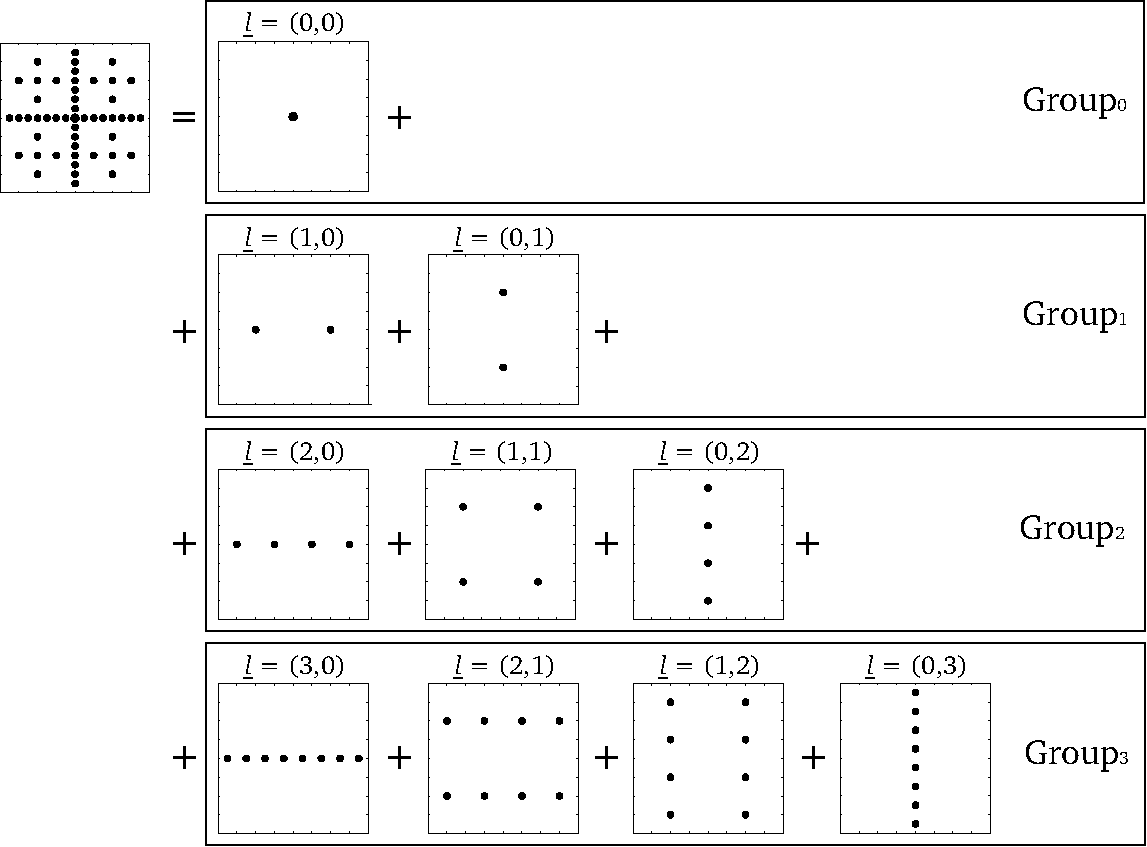
\includegraphics[width=0.9\textwidth]{truncated_sparse_grid_deco_1.pdf}
    \caption{Regular sparse grid.}
    \label{fig:truncated_sparse_grid_deco_1}
  \end{subfigure}
  \\ \\
  \begin{subfigure}[b]{1\linewidth}
    \centering
    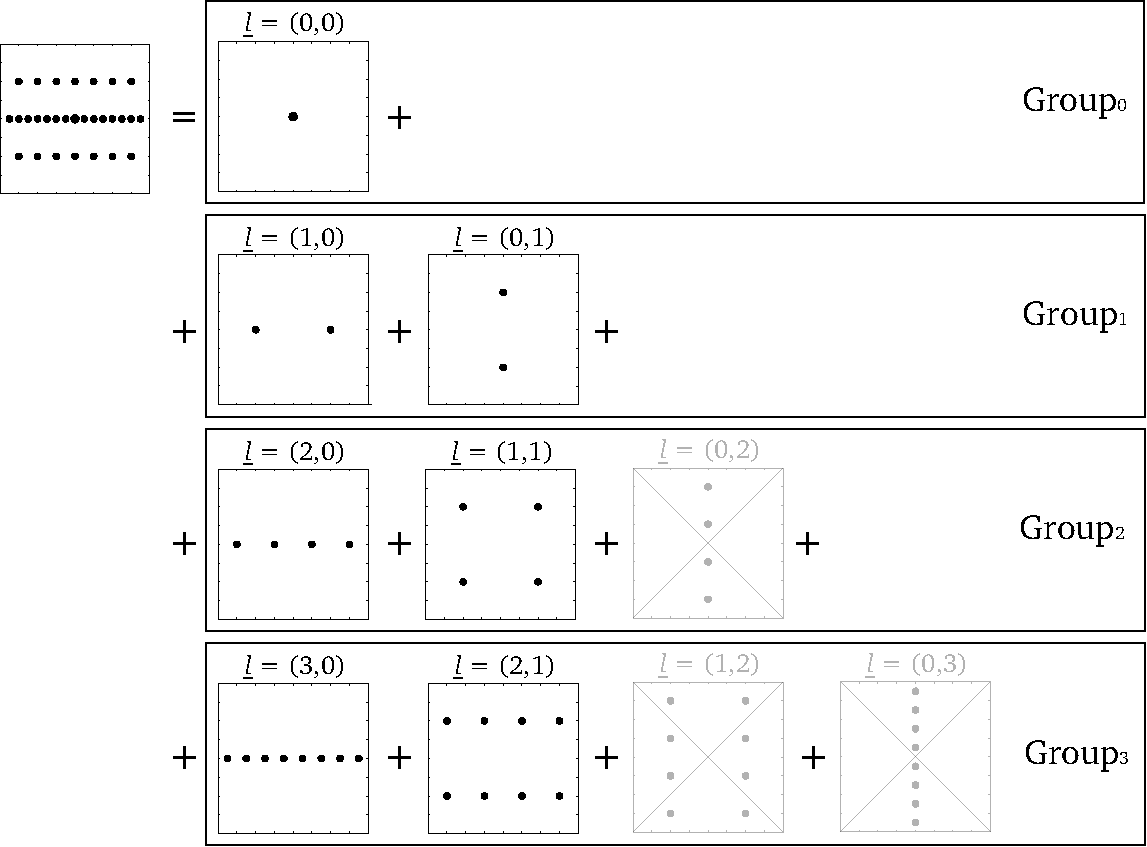
\includegraphics[width=0.9\textwidth]{truncated_sparse_grid_deco_2.pdf}
    \caption{Dimensionally truncated sparse grid.}
    \label{fig:truncated_sparse_grid_deco_2}
  \end{subfigure}
  \caption{Decomposition of regular and dimensionally truncated 2D sparse
  grids.}
  \label{fig:truncated_sparse_grid_deco}
\end{figure}

\subsection{Compression}

It is important that sparse grids should not be confused with sparse matrices.
They differ in both functionality and computational behavior. As mentioned,
sparse grids allow us to approximate multi-dimensional functions. The method is
somehow related to wavelet transformation technique \cite{Mallat89atheory},
where the computing and grouping the coefficients leads to different levels of
compression and thus an incremental representation. Similar to wavelet
compression, we also have here a hierarchical representation which corresponds
to different levels of detail. The contribution of the coefficients reduces as
this compression level increases.

Compression the multi-dimensional function means computing the hierarchical
coefficients, in a traditionally recursive manner by collecting the
contributions of all points and evaluating the basis functions in each
dimension. Using the data structure and bijection mentioned above, we can use an
iterative memory-bound algorithm for compression which is also suitable for
GPUs.

Fig.~\ref{fig:truncated_sparse_grid_deco_1} shows how a sparse grid can be
represented as a sequence of regular grids, grouped by their norm into several
refinement levels, which we'll call them \textit{groups} from now on. The grids
in one \textit{group} will be referred as \textit{blocks}. Instead of using the
traditional approach of storing the grids in trees and hash-tables, we are using
bijection based data structure with minimum memory footprint
\cite{Murarasu:2011:CDS:1941553.1941559}, which maps all $(\bar{l},\bar{i})$
pairs to consecutive integer indices. Thus, all hierarchical coefficients of the
grid will be stored efficiently in a 1-dimensional array.

\subsection{Decompression}

Interpolating at a given $D$-dimensional point means traversing the set of
regular grids and computing the contribution of each regular grid on the result. For
each regular grid a $D$-linear basis function ($\mathcal{O}(D)$) is built and
evaluated at the point. Interpolating at one point uses exactly one value from each
regular grid for scaling the basis function. Using this knowledge, we can now
look at the influence of the inputs on performance. All of these parameters
influence to some extent the performance behavior of interpolation, especially
on the GPU.

Sparse grid interpolation has 5 input parameters: the number of dimensions
($D$), the refinement level ($L$), the number of interpolations ($N$), the
precision ($P$) (single or double precision), and the truncation ($T$)
(dimensionally truncated or regular). In this paper we concentrate on the first
3, these being the most important as they can take a wide range of values.

$D$ increases the computational intensity, i.e. the ratio between the on-chip
computation time and off-chip communication time. On GPU, a large $D$ causes an
increased consumption of shared memory per thread reducing the benefits of
multithreading. A large $L$ decreases the computational intensity since the size
of the regular grids increases exponentially, i.e. from $2^0$ to $2^{L-1}$. 

As only one regular grid value is used per interpolation, only a small
percentage of the compressed data transferred over PCIe to the GPU is actually
used for computation. $N$ is proportional to the computational intensity, i.e
the more interpolations we perform, the more worthwhile is the data transfer over
PCIe.

The dimensional truncation parameter gives the possibility of reducing the
computational effort when using functions where not all input variables carry
equal weight. Therefore, instead of storing all regular grids, we can exclude
some of them when the information on those dimensions is not critical (see Fig.
\ref{fig:truncated_sparse_grid_deco_2}). In our case, this translates to
restricting the components of the $\bar{l}$ vector. An analogy can be made with
image compression. Usually images are not squares, but rectangular in shape,
having the width twice the size of their height. Going back to our sparse grids
domain, we can thus use a refinement level in one dimension (width) equal to 2x
the refinement level in the other dimension (height).

Our versions of interpolation are based on the iterative algorithm from
\cite{Murarasu:2011:CDS:1941553.1941559} over which we applied a series of
optimizations for both CPUs and GPUs. Having these two versions of
interpolation, we combine them so that all the processors in a heterogeneous
system simultaneously work on interpolation. In general, on the systems where we
measured the performance of interpolation, the GPU was faster than the CPU. But,
since our goal is performance portability, it makes sense to consider the
situation in which the GPU is not faster than the multi-core CPUs available in
the system. This can be the case for instance with Intel's Sandy Bridge
processors which have a SIMD unit~\cite{avx} (256~bit AVX) twice as wide as the
previous generation, Nehalem (128~bit SSE).

\section{Optimizations for Multi-core CPUs}
\label{sec:optimizations}
% caches: more cores -> numa -> you need locality for scalability
% vectorization: wider simd unit on cpus has to harnessed
% reducing the number of integer operations: a high number of int ops / mem ref can hide locality issues; our objective is to find and eliminate redundant int ops in our algorithms
% lines of code
% discussion about compiler vs human optimizations
% the lessons learned in this work can be of interest to a wider audience: for maximum performance, a programmer shouldn't rely solely on the power of compilers; still compilers are evolving (polyhedral model) and their evolution should be monitored; a set of representive benchmarks should be collected (human versus the compiler); of course the compiler should have access to all information a human has (no aliasing, typical data sizes (loop trip counts) when not obvious, typical data content, etc.); the optimizations we applied to our code were not found by the compilers (gcc and icc) either due to the complexity of the code or to the lack of information; our optimizations include: invariant code motion, loop exchange, loop unroll-and-jam, software pipelining, vectorization; a obvious trend in increasing the ILP of one core comes from widening the vector unit; nehalem - sse, sandy bridge - avx, g80 and gt200 - 8 simd lanes, gf100 - 32 simd lanes, knights ferry - 16 simd lanes (http://www.hpcwire.com/hpcwire/2010-08-05/compilers_and_more_knights_ferry_versus_fermi.html); such simd units cannot be ignored by a performance oriented programmer; the options here are: to rely on the compiler to automatically vectorize or to take vectorization in his or her own hands; it is important here to understand what are the factors that inhibit automatic vectorization; two examples whould be dependence analysis (aliasing, complex subscript expression, etc.) and program semantics (commutative vs non-commutative ops); moreover (cite "a guide to vectorization ...") vectorization is typically achieved by looking on the most inner loop; if the most inner has dependent iterations and the compiler doesn't perform unroll-and-jam to inject independent iterations from one of the outer loops the code cannot be vectorized; moreover the layout of the data does not favor vectorization (see sparse grid interpolation), it is unlikely that the compiler would fix that; the bottom line is that a corrent methology would be: (1) read the vectorizer report and the vectorization inhibitors, (2) eliminate the inhibitors using program transformations or compiler hints, (3) check report and if vectorization still not possible perform manual vectorization using techniques such as: loop unroll or loop unroll-and-jam, software pipelining; there are many options for manual vectorization: intrinsics sse and avx, vector types in opencl, array notations since icc v12, library approaches such a intel arbb; intrinsics offers the most flexibility but: changing to float to double, 32 bit int to 64 bit int requires code transformations (different intrinsics); moreover simd instructions are continously evolving: sse1, sse2, sse3, sse4, avx (each phase can generate a rethinking of the code, not future proof); for integer in particular: no div, no mod, 4 int x 4 int = 2 x 64 bit int, no int in avx; the solution comes from higher level abstractions; opencl seems the most promising since it is a standard but it is also a new programming model; array notations are promissing since allow for a more clear transformation of the code by simply promoting scalar variables to vector types (but it is supported only by the intel compiler); intel arbb is another promising candidate, this time a library solution not bound to a given compiler? 

Most optimizations applied to numerical codes focus on loops since these are the places where most of the execution time is spent. In general, we expect the compiler to handle loop transformations. An overview of loop transformations performed by the compiler is presented in \cite{bacon1994}. We cover in our paper only a subset of those optimizations relevant for our discussion and our routines. Specifically, we focus on optimizations that exploit the deep memory hierarchy of modern CPUs, that make use of the instruction parallelism provided by the hardware, and those that decrease the number of instructions executed.

A developer that aims at obtaining maximum performance from an architecture should not rely solely on the compiler for optimizations. In defense of this statement, we refer to the loop tiling transformation. Loop tiling is a loop reordering transformation primarily used to improve cache reuse. In loop tiling, the iteration space is divided in tiles. The transformation is highly dependent on the memory hierarchy. Aggressive tiling is done for all the levels of memory, including registers, Level-1 cache, Level-2 cache, etc. The complexity of caches complicates compiler's task to produce efficient loop tiling transformations. This is actually what motivates the existence of auto-tuners that aim to better match tile sizes with the memory levels. In the same category of loop transformations that enhance locality, there is also loop interchange. This is a transformation that exchanges the position of two loops so that the access to memory is improved, i.e. fewer cache and TLB misses. Sometimes, because the number of iterations of a loop is not known at compile time, the compiler cannot determine the best permutation of loops. Complex data dependencies resulting from complex array subscripts can also limit the applicability of this optimization since the compiler needs to prove that a given optimization preserves the semantics of the unoptimized code. This is actually a general rule followed by all compiler transformations.

Among the loop restructuring transformations that increase the instruction parallelism we find loop unrolling, loop unroll-and-jam, and software pipelining. Loop unrolling replicates the body of a loop a number of times referred to as the unrolling factor. This optimization also reduces the loop overhead and can improve the register, cache, and TLB locality. Another advantage is that more possibilities for reordering instructions are available, thus resulting in a better utilization of the instruction pipeline. The main disadvantage comes from increased size of the compiler generated code which puts more pressure on the instruction cache. Loop unroll-and-jam is similar to unroll in the sense that it copies the body of one of the next inner loops some number of times equal to the unroll-and-jam factor. The generated inner loops are then fused together (or jammed). This transformation can lead to more independent instructions in the inner loop. Software pipelining implies reordering instructions from different iterations of a loop such that independent instructions are executed in sequence. This transformation is often used in combination with loop unrolling.

In the recent period, vectorization has been gaining increased attention from developers. The current generation of processors from Intel, Sandy Bridge, contains 8-lane SIMD units (AVX), providing two times more throughput than the previous 4-lane SIMD units (SSE). Developers are interested to make use of the potential 8-fold speedup. In theory this can be achieved through vectorization performed by compilers. However, there are several factors that limit compilers' ability to vectorize a loop. As with other optimizations performed by compilers, it is important for compilers to get a correct view of data dependencies before deciding to vectorize a loop. Using pointers can create aliasing problems which reduce compilers' ability to perform data dependence analysis. Hence it can drastically limit the potential for optimizations, including vectorization. Moreover, complex expressions used as array subscripts further complicate the data dependence analysis. In general, vectorization also requires stride-1 accesses to memory in order to be efficient. As another important point, we mention that vectorization is built on top of other loop transformations. Sometimes the compiler does not reorder the loops and this does not allow for the innermost loop to be vectorized. 
% This can happen in the case of conflicting optimizations, for instance when loop reordering leads to a worse cache exploitation despite of an exploitation of the vector units. 
We do not provide here a detailed description of vectorization. Instead, we simply want to emphasize that it is an important optimization nowadays. Similar to the optimizations that target caches, human intervention is sometimes required to cope with the vectorization inhibitors. We refer the reader to \cite{vec_guide} for a complete vectorization guide for \textit{icc}. 
% A detailed guide for vectorization using \textit{icc} is available in \cite{vec_guide}.

Another important loop transformation is loop invariant code motion. This is a data-flow based loop transformation that moves outside a loop the computation whose result does not modify between iterations. 
% In such a case, the computation can be moved outside the loop, thus decreasing the number of instructions executed.
The obvious consequence is that the number of instructions executed decreases. 
We show in the following that for complex codes, it is difficult for the compiler to identify loop invariant computations. Therefore, it is essential for performance that the programmer is aware of this transformation and can apply it to the code whenever necessary. 

% It is difficult to define a clear boundary between human and compiler transformations. Probably the best methodology is to override or complement compiler produced optimizations only when it fails to apply the best code transformations. This can be achieved for instance via optimization reports generated by compilers. If these reports are not available, an advanced programmer can always check the asembly code resulting from compilation. Although this is the best practice, a trial-and-error approach can be in some situations the most productive, offering a better tradeoff between the performance achieved by the code and the time invested in optimizing it.

% It is difficult to define a clear boundary between human and compiler transformations. Building a library further complicates the process of optimizing a code. Indeed sometimes we have to take control over optimizations.

It is difficult to define a clear boundary between human and compiler produced transformations. It is often necessary for the programmer to complement or override compiler produced optimizations in order to improve the performance. But discovering missing or inefficient transformations performed by the compiler is often a tedious task. Optimization reports  generated by compilers or assembly annotated source codes help in this sense. Building a library further complicates the process of optimizing a code. 
% We can refer to this as human - compiler software codesign. 
In a library, we need to reason about the influence on performance of different values for the input parameters. Typically, it is difficult for a compiler to achieve this. A human on the other hand can address the situation by building decision trees which lead to different optimizations depending on the values of the inputs.

With these ideas in mind, we now look at three situations in which we illustrate inhibitors for compiler optimizations. To increase the performance, these inhibitors have to be addressed by the programmer. Note that the computation and memory access patterns from these examples are similar to the patterns from \textit{fastsg}'s routines.

\floatname{algorithm}{Example}
\setcounter{algorithm}{0}

\begin{figure}[tbp]
\begin{minipage}[t]{\textwidth}%
\vspace{0cm}%
\begin{minipage}[c]{0.32\textwidth}%
\vspace{0cm}%
\begin{center}
\begin{algorithm}[H]
\small{
%\caption{Loop example 1.}
 \caption{}
 \label{alg:example1}                       
 \begin{algorithmic}[1]
    \FOR{$i=1$ to $m$}
		\FOR{$j=1$ to $n$}
			\STATE $a[i] \leftarrow \text{op}(a[i], b[j], c[j])$
		\ENDFOR
    \ENDFOR
 \end{algorithmic}
}
\end{algorithm}
\end{center}
\end{minipage}%
\hfill
\begin{minipage}[c]{0.32\textwidth}%
\vspace{0cm}%
\begin{center}
\begin{algorithm}[H]
\small{
% \caption{Loop example 2, a specialization of Alg.~\ref{alg:example1}.}
 \caption{A specialization of Ex.~\ref{alg:example1}.}
 \label{alg:example2}                       
 \begin{algorithmic}[1]
    \FOR{$i=1$ to $m$}
		\FOR{$j=1$ to $n$}
			\STATE $a[i] \leftarrow a[i] \cdot b[j] + c[j]$
		\ENDFOR
    \ENDFOR
 \end{algorithmic}
}
\end{algorithm}
\end{center}
\end{minipage}%
\hfill
\begin{minipage}[c]{0.32\textwidth}%
\vspace{0cm}%
\begin{center}
\begin{algorithm}[H]
\small{
% \caption{Loop example 3.}
 \caption{}
 \label{alg:example3}                       
 \begin{algorithmic}[1]
    \FOR{$i=1$ to $m$}
		\FOR{$j=1$ to $n$}
			\FOR{$k=1$ to $p$}
				\STATE $a[i] \leftarrow a[i] \cdot b[j][k] + c[i][k]$
				\STATE $d[i] \leftarrow d[i] \cdot e[i][k] + f[j][k]$
			\ENDFOR
		\ENDFOR
    \ENDFOR
 \end{algorithmic}
}
\end{algorithm}
\end{center}
\end{minipage}%
\end{minipage}%
\end{figure}

\setcounter{algorithm}{1}
\floatname{algorithm}{Algorithm}

In Ex.~\ref{alg:example1} we can see a nest of two loops. We discuss in this context about loop interchange. For best cache exploitation, we want to have as the innermost loop the loop with fewer iterations since the number of iterations are in direct connection with the size of the arrays. Let $m$ and $n$ be bigger than the size of the cache. Since $m$ and $n$ are not known at compile time, we have to consider two situations: $m \gg n$ and $m \ll n$. In the first case, we can leave the nest in the original form. In the second one, for optimal cache usage, the loops have to be permuted, i.e. the $j$ loop is placed before the $i$ loop. This example shows that the input parameters, $m$ and $n$, influence the optimizations. A simple decision tree is built for representing input dependent optimizations. 
% Note that we do not consider in our discussion scenarios in which the computation depends on the actual content of the data.

In Ex.~\ref{alg:example2} we use the same reasoning based on the values of $m$ and $n$. If $m \gg n$, the loops do not swap places. In the current form, the innermost loop cannot be vectorized. To vectorize this loop, we perform loop tiling on the $i$ loop which is equivalent to creating two loops: $\textit{i1}$ that loops over the tiles and $\textit{i2}$ that loops inside a tile. By interchanging the $\textit{i2}$ and $j$ loops, the $\textit{i2}$ loop becomes the innermost loop, and after unrolling it using a factor of 4 for SSE (or 8 for AVX) can be easily vectorized. In the second case,  $m \ll n$, interchanging the $i$ and $j$ loops results in correct exploitation of both caches and vector units. 

Ex.~\ref{alg:example2} has \Otime{m \cdot n} complexity. In this particular example we can reduce the complexity to \Otime{m + n}. Let us observe first that for $a[i]$ we have the formula $a[i] = a[i] \cdot u + v$, where $u := \prod_{j=1}^n b[j]$ and $v := \sum_{j=1}^{n-1} ( c[j] \cdot \prod_{k=j+1}^n b[k]) + c[n]$. This means that $u$ and $v$ can be computed in the $j$ loop whereas computing $a[i]$ can be placed immediately after the $j$ loop. Note that the formulas for $u$ and $v$ contain no $i$, meaning the $j$ loop is now invariant relative to the $i$ loop, i.e. we can move it before the $i$ loop resulting in \Otime{m + n}. Experiments performed with \textit{gcc} and \textit{icc} show that these compilers cannot reduce the complexity to \Otime{m + n} even when the values for $m$ and $n$ are constant. We emphasize once more that in our scenario $m$ and $n$ are not known at compile time and in general we do not expect the compiler to manage efficiently such situations.

In Ex.~\ref{alg:example3} we consider the scenario where $n \gg m \gg p$. In response to the relation between the number of iterations of the loops, we permute the loops from $(i,j,k)$ to $(j,i,k)$ to improve locality. But, in this configuration, the innermost loop, $k$, cannot be vectorized due to data dependencies. We can apply the same method as for Ex.~\ref{alg:example2}. We perform loop tiling on the $i$ loop, thus obtaining the loops $\textit{i1}$ and $\textit{i2}$. We then move the $\textit{i2}$ loop after the $k$ loop. Since we know that $a[i]$ and $d[i]$ are independent, we can perform loop unrolling and software pipelining on the $\textit{i2}$ loop to expose the data parallelism necessary for vectorization. The last challenge comes from the data access which for the matrices $c$ and $e$ is not stride-1. This is an inhibitor for vectorization. It requires a change in the data layout for $c$ and this is again difficult to achieve only by the compiler. Therefore, the programmer needs to transform $c$ to $\tilde{c}$ according to $c[i][k] \rightarrow \tilde{c}[(i/\textit{m2}) \cdot p + k][i \bmod \textit{m2}]$, where $\textit{m2}$ is the number of iterations of the $\textit{i2}$ loop or the tile size. The same discussion applies also to matrix $e$. The access to $\tilde{c}$ and $\tilde{e}$ is now stride-1 and the innermost loop can be vectorized. Let us look again at the issues addressed in this example: unknown number of iterations and vectorization unfriendly data layout. Note that vectorization can also be achieved through unroll-and-jam applied to the initial loop $i$ after the permutation. Nevertheless, these are solutions difficult to implement by a compiler.

With this introduction in human - compiler collaborative tuning, we move to the next part of the paper that describes the strategy taken for optimizing \textit{fastsg}'s routines. 


\section{Optimization Strategies}
\label{sec:op_strategies}

The computational core of \textit{fastsg} resides in \textit{hierarchize} and
\textit{evaluate} routines. We will not enter here into the details of these
procedures because a summary is already available in \cite{murarasu2011}.
Instead, we present a set of optimizations for both of them in the context of
CPUs and GPUs. We group these optimizations into 3 categories based on their end
purpose: memory locality, vectorization, and operations with integers.

We start with a basic version of \textit{hierarchization} algorithm for GPU
where we loop with $t$ variable over all dimensions, with $g$ variable over all
\textit{groups} and then we call the kernel procedure. Each warp on the GPU
computes the coefficients for one \textit{block} of the sparse grid in order to
achieve a better cache locality and to reduce the thread divergence within
warps. Because the coefficients for one \textit{block} are stored contiguously
in memory, we also want for these values to be accessed simultaneously.
Therefore, each thread within a warp starts reading at index equal to its lane
and then subsequently every element found at a distance multiple of 32 (the
number of threads within a warp). In this way, a warp will access the memory
contiguously at each read instruction with an increased throughput. Here $l$ and
$i$ are the \textit{levels} and respectively \textit{index} vectors which
represent the coordinates of one point in the grid. We store them in the shared
memory because they are frequently used. The routines \textit{left} and
\textit{right} return the left and respectively right parents (\textit{blocks}
that the current one depends on) of a point in dimension $t$, while
\textit{agp2idx} returns the index where point $(l, i)$ is stored in the 1d
representation of the sparse grid, $asg1d$.

\begin{algorithm}[H]
\small{
	\caption{Hierarchization on GPU.}
 	\label{alg:hierarchization}                       

 	\begin{algorithmic}[1]
 		\For{$t=1$ to $D$}
 			\For{$g=L$ downto $1$}
 				\State \Call{HierarchizeKernel}{$t, g$}
 			\EndFor
 		\EndFor
 		\algstore{bkbreak}
	\end{algorithmic}
 
	\begin{algorithmic}[1]
  		\algrestore{bkbreak}
  		\Procedure{HierarchizeKernel}{$t, g$}
	 		\For{$j \leftarrow \Call{BlockStart}{g} + lane; j < \Call{BlockEnd}{g}; j\leftarrow j + 32$}
	 			\If{$lane = 0$}
	 				\State $l \leftarrow idx2l(j)$
	 			\EndIf
	 			\State $i \leftarrow idx2i(j)$
	 			\State $(\textit{ll}, \textit{il}) \leftarrow \text{left}(l, i, t)$
	 			\State $(\textit{lr}, \textit{ir}) \leftarrow \text{right}(l, i, t)$
	 			\State $\textit{v1} \leftarrow \textit{asg1d}[\text{agp2idx}(\textit{ll},
	 			\textit{il})]$ \State $\textit{v2} \leftarrow
	 			\textit{asg1d}[\text{agp2idx}(\textit{lr}, \textit{ir})]$ \State$\textit{asg1d}[j] \leftarrow \textit{asg1d}[j] - (\textit{v1} +\textit{v2}) \cdot 0.5$
			\EndFor
		\EndProcedure
	\end{algorithmic}
}
\end{algorithm}

We now optimize this basic algorithm and we start with optimizations for integer
operations. The first observation we make is that computing the $l$ vector for
each point in the \textit{block} is redundant because within a \textit{block},
it has the same value. Therefore loop invariant code motion optimization
\textit{inv1} moves the computation of $l$ outside the loop. 

Next, in \textit{inv2} we can compute for each \textit{block} of norm $g$ the
indices in $asg1d$ of all $g-1$ parent \textit{blocks} before the innermost
loop. We store them in an array (in the heap space in the case of CPU
implementation and in the shared memory of a CUDA multiprocessor for the GPU
version). To get the values for these parent points, we can now use this array
to index $asg1d$ and get the \textit{block}. What we still need is the index
inside the \textit{block}. This is computed inside the $j$ loop by converting
$i$ to the corresponding index.

\textit{inv3} starts from the observation that $\tilde{l}$ and $\tilde{i}$, the
\textit{levels} and respectively \textit{index} vectors of the parents, differ
from $l$ and $i$ of the current point only in one dimension. Therefore, the
conversion mentioned above is not necessary anymore, thus reducing the
complexity from $O(D)$ to $O(1)$.

Now, in the innermost loop over the current \textit{block}, what is left to
compute is the conversion $(l(t), i(t)) \rightarrow (\tilde{l}(t),
\tilde{i}(t))$ which has a complexity of $O(l(t))$. \textit{inv4} precomputes
the results of these conversions before the kernel launch and stores them in an
array. The advantage is that the complexity of the innermost loop is now $O(1)$,
but at a cost of higher memory footprint.

Lastly, in order to improve memory locality and the data access patterns,
\textit{ichg1} optimization does a loop interchange by moving the loop over the
\textit{groups} from line 2 inside the kernel. In this way, one warp will not
only process one \textit{block}, but also all its parents.

% We start with the algorithm for hierarchization. In this algorithm,
% \textit{asg1d} is a 1d array containing the values of a dimensionally adaptive
% sparse grid. We traverse \textit{asg1d} $d$ times, each time updating the value
% at a point based on the values of its dependencies, i.e. its parents, in the
% current dimension, $t$. The iterations of the $t$ loop
% % \footnote{We refer to loops using their respective loop counters.} 
% are dependent. The $g$ loop traverses \textit{groups} of grid points whereas the
% $b$ loop iterates over \textit{blocks} from the same group. Finally, the $k$
% loop is equivalent to the traversal of all the points of a \textit{block}.
% 
% The left and right parents of a point in dimension $t$ is returned by the
% routines \textit{left} and \textit{right} respectively. Computing the left
% parent in dimension $t$ is equivalent to solving the equation $(i_t - 1) \cdot
% 2^{-l_t} = \textit{il}_t \cdot 2^{-\textit{ll}_t}$, where $\textit{il}_t \in
% \{1, \dots, 2^{\textit{ll}_t+1}\}$ and $\textit{il}_t$ odd. Except for the
% $t$-th components, all the other components of $\textit{ll}$ and $\textit{il}$
% are equals to the ones of $l$ and $i$ respectively. Similarly, the right parent
% is given by $(i_t + 1) \cdot 2^{-l_t} = \textit{ir}_t \cdot 2^{-\textit{lr}_t}$.
% All its other components are the same as in $l$ and $i$. An important
% observation is that for both the left and right parent $\textit{ll}_t < l_t$ and
% $\textit{lr}_t < l_t$.
% 
% Understanding the parent concept is essential for understanding the cache
% locality of this algorithm. We first need to look at dependencies from a higher
% level. Remember that in our data layout, we pack the grids points in
% \textit{blocks}. The identifier of a \textit{block} is the $l$ shared by the
% points it contains. For any \textit{block} with the norm of its identifier $b$,
% the parents of its points reside in $b - 1$ blocks with the same components of
% their respective identifiers except the $t$-th. We can therefore say that the
% dependencies of the \textit{block} reside in a relatively compact memory space
% with a total size of $2^b - 1$, where $2^b$ is the size of the \textit{block}.
% This result invalidates part of the analysis presented in \cite{murarasu2011}
% that presents \textit{hierarchization} as a cache unfriendly operation. Note
% that the cache optimization is a direct benefit of the storage scheme.
% 
% In Alg.~\ref{alg:hierarchization} a considerable amount of time is spent
% computing the bijections, \textit{idx2agp} and \textit{agp2idx}. Our first two
% optimizations, \textit{opt1} and \textit{opt2}, target exactly this problem.
% They perform loop invariant code motion, placing operations from the bijections
% immediately before the innermost loop. \textit{opt1} is based on the observation
% that all the points in the same \textit{block} have the same $l$. Hence $l$ can
% be computed only once for any \textit{block} with $2^g$ points. This means it is
% safe to move the computation of $l$ from line 6 outside the $k$ loop.
% \textit{opt2} relies on the fact that a \textit{block} whose identifier has the
% norm $g$ has $g - 1$ \textit{block} dependencies. This means that we can compute
% the indices in \textit{asg1d} of these \textit{blocks} immediately before the
% innermost loop and store them in a small 1d array, $\textit{idx12mem}$ of size
% $n$. By doing so, we reduce the number of operations in lines 9 and 10. Remember
% that the bijection computes three indices. With this optimization only
% $\textit{idx3}$ has to be computed in the body of the $k$ loop. The sum
% $\textit{idx1} + \textit{idx2}$ is obtained by indexing $\textit{idx12mem}$
% using the $t$-th component of $\textit{ll}$ in line 9 and $\textit{lr}$ in line
% 10. In Sec.~\ref{sec:evaluation} we show that we cannot obtain this optimization
% automatically from compilers. Summarizing the results, we can say that
% \textit{opt1} provides a speedup of 1.75 over the basic (unoptimized) version.
% \textit{opt1} and \textit{opt2} accelerate together the routine approximately
% 3.75 times.
% 
% Our third optimization, \textit{opt3}, reduces the number of instructions
% executed in line 6. After moving the computation of $l$ outside the loop, in
% line 6 there is only $i$ to compute. This is the inverse of the operation that
% computes $\textit{idx3}$ (Formula~\ref{eq:idx3}). The complexity of this
% operation is \Otime{d}. We replace it with an iterator that generates the
% current $i$ based on the previous $i$. The central concept of the iterator is
% the following. It increments the values of $i$ starting with the last component
% until no carry is generated or there are no more components left. A carry is
% produced when the $t$-th component of $i$ reaches the value $2^{l[t]}$. Whenever
% a carry is generated, the corresponding component of $i$ is reset to zero. Our
% results show that \textit{opt3} accelerates the version of
% \textit{hierarchization} optimized with \textit{opt1} and \textit{opt2} up 1.5
% times. Note that \textit{opt3} introduces dependencies between the iterations of
% the innermost loop.
% 
% In our fourth optimization, \textit{opt4}, we manually unroll the $k$ loop in
% order to allow for vectorization in the implicit loops from the lines 6, 9, and
% 10. This optimization is incompatible with \textit{opt3} since \textit{opt3}
% makes the iterations of the $k$ loop dependent. Therefore, we apply this
% optimization only on top of \textit{opt1} and \textit{opt2}. For vectorization,
% we use in \textit{opt4} SSE intrinsics for integer operations. We show in
% Sec.~\ref{sec:evaluation} that the benefit of \textit{opt4} depends highly on
% the compiler used. In general, our results show that \textit{opt3} performs
% better than \textit{opt4}.

We move now to the algorithm for \textit{evaluation}. The coordinates of all $N$
points to be evaluated are stored contiguously in a matrix $x[N][D]$ which is
processed in chunks by each warp, each warp computing one chunk of size $w$. The
memory access pattern for one thread inside of its chunk is the same as for
\textit{hierarchization} algorithm where each thread computes points stored at
indices multiple of 32 starting from the corresponding lane. The $g$ and $b$
loops traverse \textit{groups} and \textit{blocks} respectively.
$\textit{idx23}$ is used to index the beginning of the current \textit{block} in
$\textit{asg1d}$, while $idx1$ idexes the current point in this \textit{block}.

\begin{algorithm}[H]
\small{
	\caption{Evaluation on GPU.}
	\label{alg:evaluation}
	\begin{algorithmic}[1]
 		\Procedure{EvaluateKernel}{$w$}
    		\For{$j \leftarrow \Call{ChunkStart}{w} + lane; j < \Call{ChunkEnd}{w}; j \leftarrow j + 32$} 
    		\State $\textit{idx23} \leftarrow 0$
				\For{$g=1$ to $L$}
					\For{$b=1$ to $a(D, g)$}
						\State $\textit{idx1} \leftarrow 0$
						\State $\textit{p} \leftarrow 1$
						\If{$threadIdx.x = 0$}
							\State Compute $l$ for which $\text{pos}(l) = b$
						\EndIf
						\For{$t=1$ to $D$}
							\State $i \leftarrow \lfloor x[j][t] / 2^{l[t]} \rfloor \cdot 2 + 1$
							\State $p \leftarrow p \cdot \max(1 - |2^{l[t]} \cdot x[j][t] - i|, 0)$
							\State $\textit{idx1} \leftarrow \textit{idx1} \cdot 2^{l[t]} + \lfloor	x[j][t] / 2^{l[t]} \rfloor$
						\EndFor
						\State $r[j] \leftarrow r[j] + \textit{asg1d}[\textit{idx1}	+\textit{idx23}] \cdot p$ 
						\State $\textit{idx23} \leftarrow \textit{idx23} + 2^g$
					\EndFor
				\EndFor
    		\EndFor
    	\EndProcedure
 	\end{algorithmic}
}
\end{algorithm}

We start with optimizations for a better vectorization. For the CPU version,
in \textit{vec1} we use loop unroll-and-jam, loop tiling and we vectorize the
innermost loop $t$. Software pipelining can be done in the unrolled loop, but
$x$ is accessed with stride-$D$ instead of stride-1. Therefore, we change the
layout of $x$ such that $x[j][t] \rightarrow \tilde{x}[(j/\textit{m2}) \cdot D +
t][j \bmod \textit{m2}]$, where $\textit{m2}$ is the size of the tile. Now, a
stride-1 access on $\tilde{x}$ is possible which makes SSE vectorization
efficient. For GPUs, the observation we make is that the loop over dimensions on
line 11 has a non-contiguous access pattern for a warp because at each read
instruction the threads within a warp access elements found at $D$ distance.
\textit{vec1'} improves this by using a technique similar to the one we
described for both \textit{hierarchization} and \textit{evaluation} algorithms
for increasing the throughput through memory coalescing by threads within a
warp. More specific, \textit{vec1'} transposes the matrix $x$ such that instead
of storing the the points horizontally, one point per row, it stores them
vertically in $\tilde{x}[(N/32+1) \cdot D][32]$. Thus, all threads in a warp
access one row in this new matrix for each iteration over dimensions.

Regarding memory locality, \textit{ichg2} does a loop interchange by moving the
loop over interpolation points from line 2 inside the loop over \textit{blocks}
from line 5. In the case of GPUs, we have two variations of this optimization.
The first one, \textit{ichg2'} corresponds to \textit{ichg2} while the second
one, \textit{ichg2''}, additionally moves the loops over \textit{groups}
and \textit{blocks} outside the kernel. The goal of these optimizations is to
improve read accesses by having the innermost loop as tight as possible over the
block of memory.

The last optimization is a combination of strength reduction and loop invariant
code motion introduced in order to speed up integer operations. \textit{sred1}
precomputes all divisions in lines 12-14 outside the innermost loop and replaces
them with multiplications with the inverse. In addition, $idx1 \leftarrow
idx1 \cdot 2^{l[t]} + \lfloor x[j][t] / 2^{l[t]} \rfloor$ from line 14 is
replaced with $idx1 \leftarrow idx1 + \lfloor x[j][t] / 2^{l[t]} \rfloor
\cdot 2^{prefix\_sums[t + 1]}$, where $prefix\_sums[p] = \sum_{p=t}^{D-1}l[p]$.
This makes indexing a normal reduction and increases the instruction level
parallelism.
% 
% \begin{algorithm}[tbp]
% \small{
%  \caption{Evaluation.}
%  \label{alg:evaluation}                       
%  \begin{algorithmic}[1]
%     \FOR{$j=1$ to $m$}
% 		\STATE $\textit{idx23} \leftarrow 0$
% 		\FOR{$g=1$ to $n$}
% 			\FOR{$b=1$ to $a(d, g)$}
% 				\STATE $\textit{idx1} \leftarrow 0$
% 				\STATE $\textit{p} \leftarrow 1$
% 				\STATE Compute $l$ for which $\text{pos}(l) = b$
% 				\FOR{$t=1$ to $d$}
% 					\STATE $i \leftarrow \lfloor x[j][t] / 2^{l[t]} \rfloor \cdot 2 + 1$
% 					\STATE $p \leftarrow p \cdot \max(1 - |2^{l[t]} \cdot x[j][t] - i|, 0)$
% 					\STATE $\textit{idx1} \leftarrow \textit{idx1} \cdot 2^{l[t]} + \lfloor x[j][t] / 2^{l[t]} \rfloor$
% 				\ENDFOR
% 				\STATE $r[j] \leftarrow r[j] + \textit{asg1d}[\textit{idx1} + \textit{idx23}] \cdot p$
% 				\STATE $\textit{idx23} \leftarrow \textit{idx23} + 2^g$
% 			\ENDFOR
% 		\ENDFOR
%     \ENDFOR
%  \end{algorithmic}
% }
% \end{algorithm}
% 
% We now move to Alg.~\ref{alg:evaluation} representing the core of our
% \textit{evaluate} routine. We give a brief explanation of this algorithm. The
% $j$ loop from line 1 iterates over the points where we evaluate the sparse grid.
% These points are stored in the matrix $x[m][d]$. We store the evaluation results
% in the $r$ vector. Similarly to the algorithm for hierarchization, the $g$ and
% $b$ loops traverse \textit{groups} and \textit{blocks} respectively. For every
% point represented as a row of $x$, we use exactly one value from every $block$
% (line 12). $\textit{idx23}$ is used to index the beginning of the current
% \textit{block} in the 1d representation of the sparse grid, i.e. the 1d array
% $\textit{asg1d}$.
% 
% \textit{opt5} applied to this algorithm makes some assumptions about the number
% of iterations of the loops. We know that in general $\textit{asg1d}$ can be up
% to three orders of magnitude bigger than $x$. On the other hand, $2^g$ is
% typically smaller than the size of $x$. In this context, for better locality we
% permute the loops from $(j, g, b, t)$ to $(g, b, j, t)$. Note that this
% optimization also reuses $l$ from line 6 for multiple points from $x$. Our
% results show that this improves the basic version of evaluation up to a factor
% of 2.5. It is worth mentioning that this speedup depends on the number of
% iterations of the loops. The benefits of \textit{opt5} can be more impressive if
% we increase the ratio between the size of $\textit{asg1d}$ and the size of $x$.
% 
% Even after applying \textit{opt5}, there is not too much potential for
% vectorizing the $t$ loop due to the existence of dependencies between
% iterations. Nevertheless, we build \textit{opt6} on top of the permutation from
% \textit{opt5}. We can vectorize the innermost loop, $t$, by following the steps:
% grabbing iterations from the $j$ loop, inserting them in the $t$ loop, and
% reordering the instructions such that the same instructions operating on
% different data are packed together. The first two steps are equivalent to loop
% tiling, loop interchange, and loop unrolling. The third step is software
% pipelining in the unrolled loop. This is not enough as the access to $x$ is not
% stride-1. Actually, we have a stride-$d$ access. To cope with this problem, we
% change the layout of the $x$ matrix using the transformation $x[j][t]
% \rightarrow \tilde{x}[(j/\textit{m2}) \cdot d + t][j \bmod \textit{m2}]$, where
% $\textit{m2}$ is the size of the tile from the loop tiling transformation. Using
% $\tilde{x}$ instead of $x$ we have the stride-1 access required for efficient
% vectorization. By vectorizing the \textit{evaluate} routine using SSE
% intrinsics, we accelerate the version optimized using \textit{opt5} up to 2.6
% times.
% 
% \subsection{Parallelization of Sparse Grid Operations}
% 
% Our sparse grids routines are parallelized for shared memory machines using
% OpenMP. We provide in this part a brief description of the parallelization
% scheme used in \textit{fastsg}.
% 
% Alg.~\ref{alg:hierarchization} does not offer many possibilities for
% parallelization mainly due to the sequential optimizations. The $t$ loop has
% dependent iterations. The iterations of the $k$ loop are also dependent after
% applying \textit{opt3}. Additionally, we cannot update two \textit{groups} in
% parallel as one of them can depend on the old values of the second. Remember
% that we also aim at minimal memory consumption, meaning we want to keep our
% algorithm in-order, i.e. no extra copies of the data. Considering all these
% restrictions, the only loop whose iterations can be distributed among worker
% threads is the $b$ loop.
% 
% Regarding the evaluation algorithm, we have more options for parallelization. A
% first parallelization approach is taken to cover the case when the sparse grid
% is evaluated at a small number of points, e.g. one point. It implies
% distributing the iterations of the $b$ loop. In the case of one point, at the
% end of the \textit{evaluate} routine, the results computed by multiple threads
% are summed up. We use a coarser parallelization method if the number of points
% where we evaluate the sparse grid is reasonably big, e.g. bigger than 10,000. In
% this scenario, we parallelize the $j$ loop.


\section{Evaluation}
\label{sec:evaluation}

In this section we present the results obtained for both CPU and GPU
implementations and analyze the speedup obtained when applying the
optimizations described in Section~\ref{sec:op_strategies}.

Our test system is a quad-core Intel Core i7-920 running at 2.67 GHz with
Hyper-threading enabled. For compilation we used \textit{gcc 4.6} with flags
``-O3 -march=native -funroll-loops -fargument-noalias -fopenmp''. The GPU cards
used were GeForce GTX 480 from Nvidia (Fermi architecture) having 1.5 GB of
total memory and 15 multiprocessors each with 32 lanes operating at a clock
speed of 1.4 GHz. For programming the GPUs, we started from the CPU code base
and implemented the algorithms and optimizations with the established CUDA
framework, making use of specific Nvidia features. An important observation to
make is that the device supports CUDA Capability 2.0 which, among other
features, includes the possibility for the same on-chip memory to be used for
both L1 cache and shared memory. It can be configured as either 48 KB of shared
memory and 16 KB of L1 cache or as 16 KB of shared memory and 48 KB of L1 cache.
We used the second option for the \textit{evaluation} algorithm in order to
cache the accesses to local and global memory and also temporary register
spills. For compilation, we used \textit{Cuda Toolkit 4.1} with flags
``-arch=sm\_20''.

\begin{figure}[t]
  \begin{subfigure}[b]{1\linewidth}
    \centering
    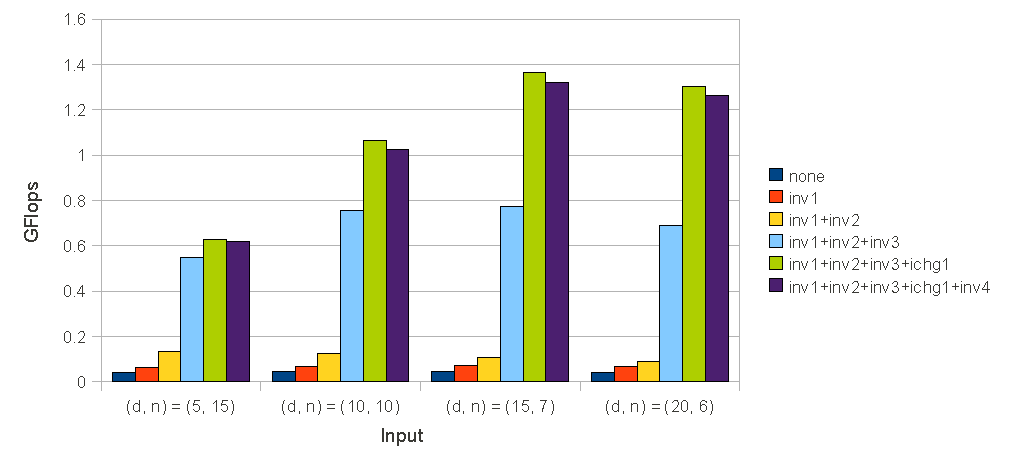
\includegraphics[width=1\linewidth]{hier_cpu} \\
    \caption{CPU}
  \end{subfigure}
  \\ \\
  \begin{subfigure}[b]{1\linewidth}
    \centering
    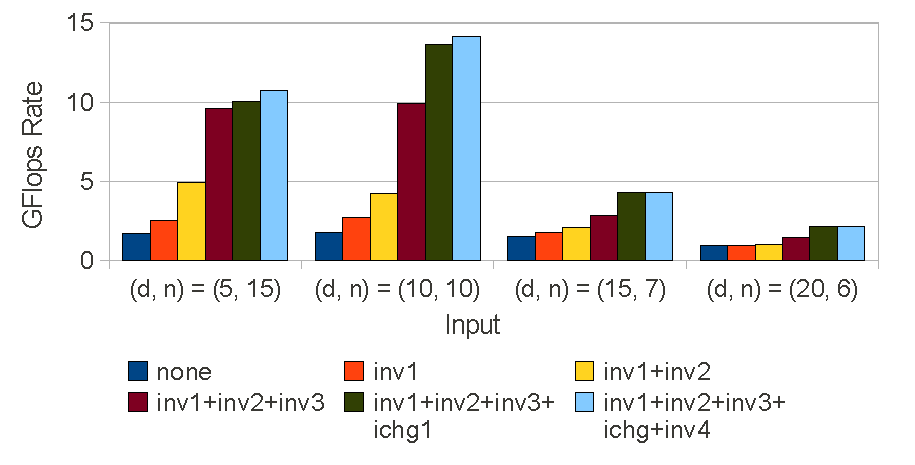
\includegraphics[width=1\linewidth]{hier_gpu}
    \caption{GPU}
  \end{subfigure}
  \caption{Impact of optimizations on the performance of \textit{hierarchization} algorithm.}
  \label{fig:hier_results}
\end{figure}

We present the impact of our optimizations for both CPU and GPU implementations
by measuring the GFlops rate and comparing with the reference baseline case
where no optimizations were applied. We start with the results obtained for the
\textit{hierarchization} algorithm, depicted in Fig.~\ref{fig:hier_results}. The
tests were done using different configurations, as displayed on the X-axis,
where $d$ is the number of dimensions and $n$ is the number of refinement
levels. We can see here that when applying all optimizations, a speedup of up to
34x is obtained for CPU and up to 8x for GPU compared to the respective baseline
cases. With the increase in the number of dimensions and the decrease of the
sparse grid size, the speedup for GPU tends to decrease. This happens because
the effects of most of the optimizations (e.g. improving caching and memory
access patterns) are visible when a high degree of parallelism is achieved,
situation which happens in the case of large grids. It is also interesting to
notice that \textit{inv4} brings a drop of performance when applied on top of
the other optimizations for CPU, although for GPU it brings a speedup. This
means that when the grids are smaller then it is better to actually do the
computations instead of doing memory lookups, which may result in cache misses.
Giving this empirical optimization, a heterogeneous system could activate or
deactivate it at runtime based on the architecture and compiler used. Lastly, we
show that a speedup of 17x is obtained for the most performant GPU version
compared to the corresponding CPU-based one and a speedup of 6.2x compared to
the state-of-the-art GPU version~\cite{Murarasu:2011:CDS:1941553.1941559}.

\begin{figure}[t]
  \begin{subfigure}[b]{1\linewidth}
    \centering
    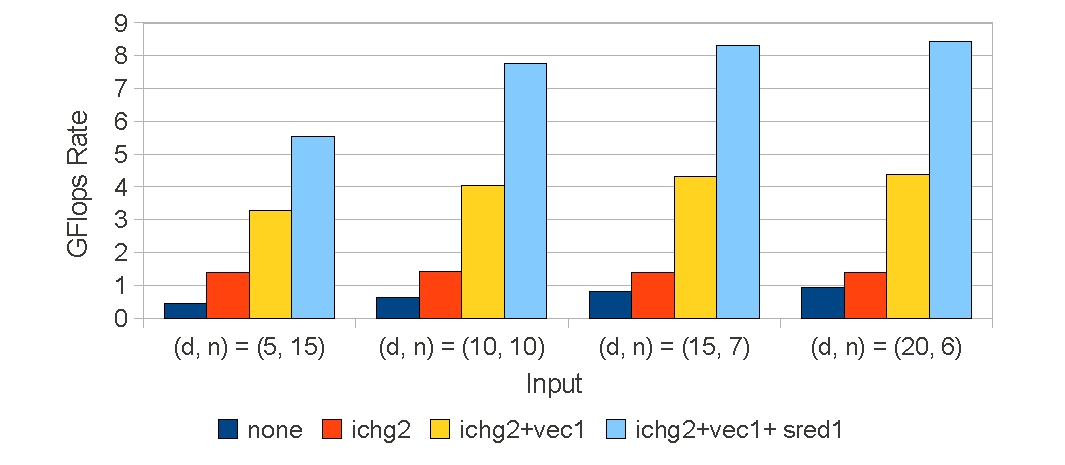
\includegraphics[width=1\linewidth]{eval_cpu} \\
    \caption{CPU}
  \end{subfigure}
  \\ \\
  \begin{subfigure}[b]{1\linewidth}
    \centering
    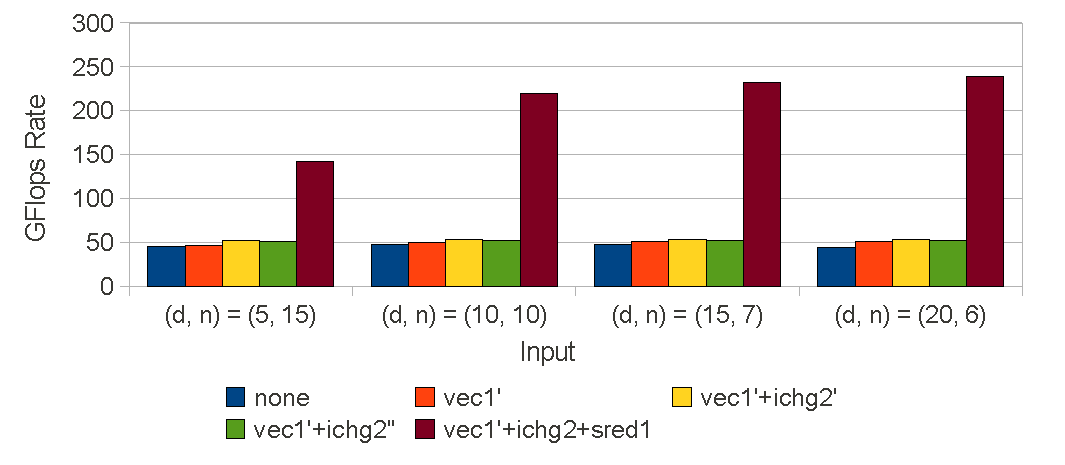
\includegraphics[width=1\linewidth]{eval_gpu}
    \caption{GPU}
  \end{subfigure}
  \caption{Impact of optimizations on the performance of \textit{evaluation} algorithm.}
  \label{fig:eval_results}
\end{figure}

For the \textit{evaluation} algorithm, we used $10^{4}$ for CPU and $10^{6}$
for GPU random points, uniformly distributed in the function domain. Here we
make two empirical observations. First, the GFlops rate for CPU remains constant
when increasing the number of interpolation points. Second, we used 8 chunk
sizes (number of interpolation points) for each warp: 32, 64, 96, 128, 160, 192,
224, and 256, but chose only the optimal one for each optimization. A pattern on
how the chunk size affects the performance could not be observed, which
motivates for a careful tunning of the algorithm before running.

The results of our tests are presented in Fig.~\ref{fig:eval_results}. Compared
to the CPU versions, the optimizations for GPU are not that effective. The main
reason for this is that giving the high memory requirement for storing the
interpolation points, we used the GPU's global memory. Although caching is
performed, we believe that a higher throughput could be obtained if we could
have stored the results in shared memory. The optimization which brings a clear
speedup is \textit{sred1} showing that division instructions are still very
expensive on GPUs, fact also emphasized by \cite{cuda}. The GPU version is 28.3x
faster than the CPU one which confirms that sparse grids interpolation technique
is cache friendly and easily parallelizable using our data structure. Compared
to the state-of-the-art GPU version~\cite{Murarasu:2011:CDS:1941553.1941559}, a
speedup of 1.5x is obtained for this algorithm.


\section{Conclusion}

In this paper we presented a series of loop transformations and showed
how they behave on CPUs and GPUs when applied to a computational steering
application. We argued that giving the architectural similitude of CPUs and GPUs
seen both as vector processors with different vector units sizes and roughly
same cache hierarchy, some optimizations, at least conceptually, should be the
same. With these concepts in mind, we proposed an extensive set of optimizations
for both CPUs and GPUs that provide a speedup of up to 12.8x and 5.2x
respectively.

In addition, we presented the first implementation of hierarchization and
interpolation algorithms for adaptive sparse grids on GPUs and proved that our
data structure and associated algorithms are easily parallelizable using
architecture independent loop transformations.

We see the convergence of CPUs and GPUs both in terms of hardware features and
programming languages. On heterogeneous systems OpenCL \cite{opencl} is slowly
making its way, but it is not as mature as CUDA and remains similarly complex.
OpenACC \cite{openacc} is a new standard with a lot of promise which focuses on
parallelization of loop nests. These types of frameworks will take the burdon
of focusing on architecural differences when programming, while at the same time
incorporating common transformations and using auto-tuning techniques for evaluation.


\bibliographystyle{IEEEtran}
\bibliography{refs}



\end{document}
